\section{Εξαγωγή αμφιωτικών παραμέτρων}

\noindent
Σε αυτή την ενότητα, αναλύεται η εφαρμογή του μοντέλου του Dietz το θεωρητικό υπόβαθρο του οποίου περιγράφεται στην υποενότητα \ref{sec:dietz_theory}. Η συνάρτηση είναι υλοποιημένη σε MATLAB, στο Auditory Modeling Toolbox. Η συνάρτηση χρειάζεται ως ορίσματα το binaural σήμα και τη συχνότητα δειγματοληψίας, ενώ στην έξοδό της δίνονται οι αμφιωτικές παράμετροι.

Συνοπτικά η διαδικασία που ακολουθείται για τον υπολογισμό των παραμέτρων, φαίνεται στο Σχήμα \ref{fig:dietz_block_diagram_MATLAB} και τα επιμέρους στοιχεία της αναλύονται στη συνέχεια.

\begin{figure}[h]
  \centering
  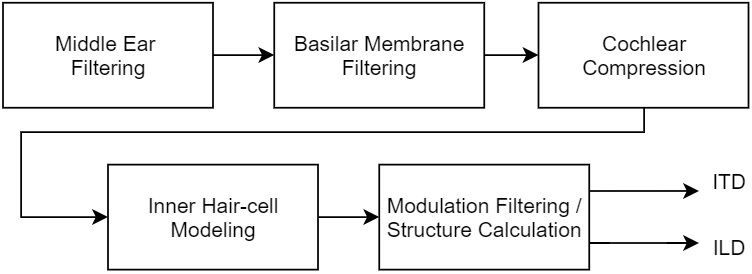
\includegraphics[width=\textwidth]{images/dietz_block_diagram_MATLAB.png}
  \caption{Συνοπτική περιγραφή της υλοποίησης του μοντέλου Dietz για το ακουστικό σύστημα.}
  \label{fig:dietz_block_diagram_MATLAB}
\end{figure}

\noindent
Αξίζει εδώ να σημειωθεί πως η υλοποίηση του μοντέλου, πιστώνεται στους:
\begin{itemize}
    \item Tobias Peters (tobias@medi.physik.uni-oldenburg.de)
    \item Mathias Dietz (mathias.dietz@uni-oldenburg.de)
    \item Martin Klein-Hennig (martin.klein.hennig@uni-oldenburg.de)
\end{itemize}{}

Παρακάτω, μελετάται η λειτουργία του μοντέλου, με βάση ένα  από τα binaural σήματα εισόδου που χρησιμοποιούνται, που αντιστοιχεί σε γωνία άφιξης $+80^o$ από το δωμάτιο Spirit, όπως φαίνεται στο Σχήμα \ref{fig:example_bin_sig}.

\begin{figure}[h]
  \centering
  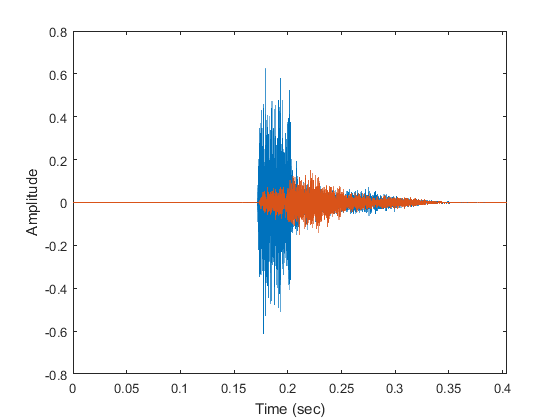
\includegraphics[width=\textwidth]{images/example_bin_sig.png}
  \caption{Binaural σήμα για γωνία άφιξης $+80^o$, στο δωμάτιο Spirit.}
  \label{fig:dietz_out}
\end{figure}

\subsection{Φιλτράρισμα Μέσου Αυτιού}

Αρχικά, το σήμα περνά από ένα bandpass butterworth φίλτρο με $f_{c1} = 500 Hz$ και $f_{c2} = 2 kHz$ το οποίο φαίνεται στο Σχήμα \ref{fig:butterworth_dietz_1}, ενώ το τελικό αποτέλεσμα της επεξεργασίας φαίνεται στο Σχήμα \ref{fig:dietz_out1}. Όπως είναι αναμενόμενο, όντας ουσιαστικά σήμα λευκού θορύβου, η μορφή του αλλάζει αισθητά στο πεδίο του χρόνου, αφού μειώνεται σημαντικά το υψίσυχνο περιεχόμενο.

\begin{figure}[h!]
  \centering
  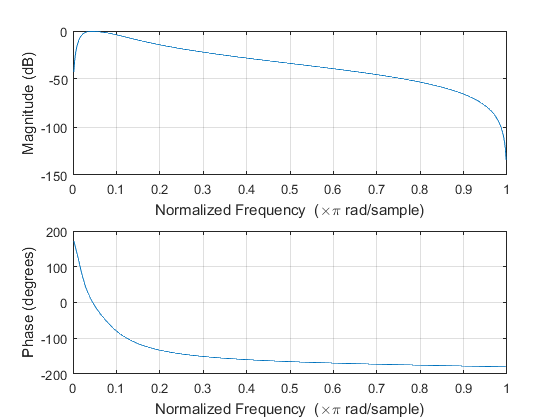
\includegraphics[width=\textwidth,height=8cm]{images/butterworth_dietz_1.png}
  \caption{IIR φίλτρο τύπου butterworth που προσομοιώνει το φιλτράρισμα του μέσου αυτιού.}
  \label{fig:butterworth_dietz_1}
\end{figure}

\begin{figure}[h!]
  \centering
  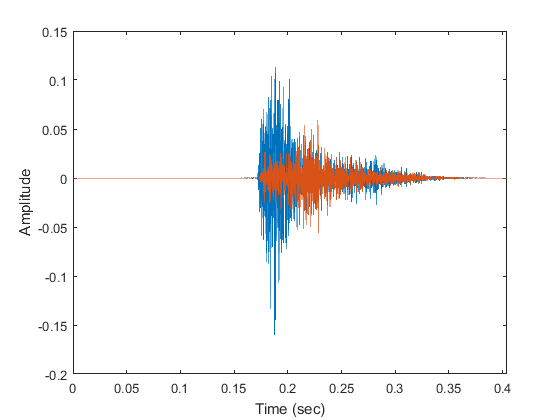
\includegraphics[width=\textwidth]{images/dietz_out1.png}
  \caption{Αποτέλεσμα της επεξεργασίας του μέσου αυτιού.}
  \label{fig:dietz_out1}
\end{figure}

\subsection{Προσομοίωση Εσωτερικού Αυτιού}

Σε αυτό το σημείο, για την προσομοίωση της basilar μεμβράνης, υπολογίζονται 23 gammatone φίλτρα με μιγαδικούς συντελεστές για τον υπολογισμό της ITF (Εξίσωση \ref{eq:ITF}). Το πλήθος των φίλτρων προκύπτει από το γεγονός ότι μεταξύ τους απέχουν 1 ERB, το οποίο αντιστοιχίζεται σε περίπου 217 Hz, και καλύπτουν το διάστημα 200 - 5000 Hz. Η κρουστική απόκριση ενός gammatone φίλτρου, περιγράφεται στην Εξίσωση \ref{eq:gammatone_IR}. Ουσιαστικά είναι ένα φίλτρο που προκύπτει από τον πολλαπλασιασμό μιας κατανομής γάμμα, και ενός ημιτονοειδούς τόνου. Οι αποκρίσεις συχνότητας των 23 φίλτρων παρουσιάζονται στο Σχήμα \ref{fig:gammatone_responses}. Το αποτέλεσμα του φιλτραρίσματος, είναι μιγαδικό, και αποτελείται από 23 συχνοτικές μπάντες.

\begin{CEquation}
    g(t) = \alpha t^{n-1}\cos{(2\pi f_c t)}e^{-2\pi\beta t}
    \label{eq:gammatone_IR}
\end{CEquation}

\begin{figure}[h]
  \centering
  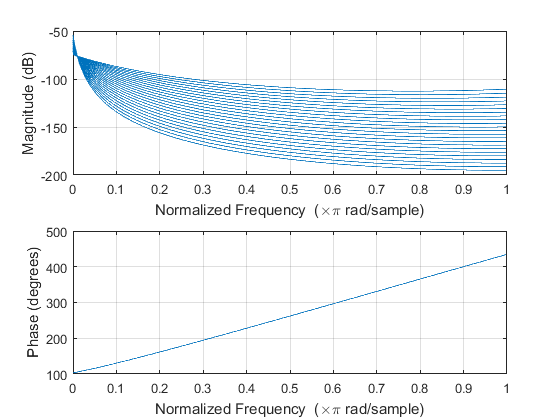
\includegraphics[width=\textwidth]{images/gammatone_responses.png}
  \caption{Αποκρίσεις συχνότητας της τράπεζας φίλτρων gammatone.}
  \label{fig:gammatone_responses}
\end{figure}

Στη συνέχεια για τη μοντελοποίηση της συμπίεσης του κοχλία χρησιμοποιείται η Εξίσωση \ref{eq:cochlear_compression} δείγμα προς δείγμα. Ακολούθως, τα εσωτερικά hair-cells του αυτιού μοντελοποιούνται όπως έχει ήδη αναφερθεί με μια ανόρθωση ημίσεος κύματος και στη συνέχεια ένα lowpass φίλτρο, με αποτέλεσμα την εξαγωγή μια 'περιβάλλουσας'. Στο σημείο αυτό, το ένα εκ των δύο καναλιών του σήματος, έχει τη μορφή που φαίνεται στο Σχήμα \ref{fig:dietz_out2}.

\begin{CEquation}
    y(n) = sign(x(n)) * |x(n)| ^ c
    \label{eq:cochlear_compression}
\end{CEquation}

\begin{figure}[h]
  \centering
  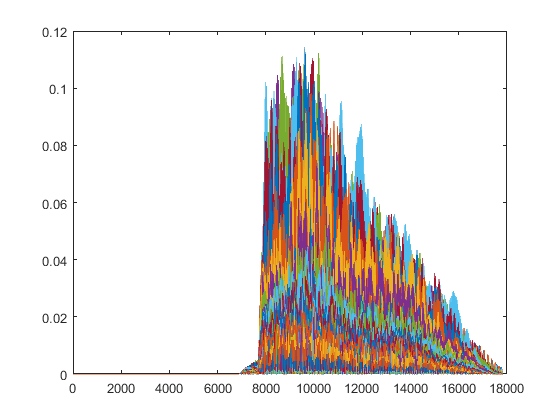
\includegraphics[width=\textwidth]{images/dietz_out2.png}
  \caption{Έξοδος του μοντέλου μετά τη μοντελοποίηση του εσωτερικού αυτιού.}
  \label{fig:dietz_out2}
\end{figure}

\subsection{Τράπεζα Φίλτρων Διαμόρφωσης}

Το επόμενο στάδιο της επεξεργασίας περιέχει ακόμα μια τράπεζα φίλτρων, που αποτελείται από τρία gammatone φίλτρα 2ης τάξης, για τον διαχωρισμό στις δομές 'fine' και 'envelope' που περιέχουν πληροφορία χαμηλών (κάτω από 1.4 kHz) και υψηλών συχνοτήτων αντίστοιχα και ένα lowpass με $f_c = 30 Hz$ για τον υπολογισμό του ILD. Κατ' επέκταση, η fine δομή έχει 12 διαστάσεις, που κάθε μια αντιστοιχεί σε συχνοτικές μπάντες από $200-1400 Hz$ ενώ η δομή envelope 11 διαστάσεις που αντιστοιχούν στις εναπομείνασες συχνότητες. Τα προαναφερθέντα φίλτρα, εφαρμόζονται σε κάθε μία από τις συχνοτικές μπάντες της εξόδου του προηγούμενου σταδίου. Οι έξοδοι σε αυτό το σημείο, λόγω των μιγαδικών συντελεστών των gammatone φίλτρων είναι πάλι μιγαδικές.

\subsection{Αμφιωτικός επεξεργαστής}

Το τελευταίο στάδιο της επεξεργασίας, υλοποιείται από τον binaural processor, o οποίος εφαρμόζει τις εξισώσεις που έχουν περιγραφεί αναλυτικά στο κεφάλαιο \ref{sec:dietz_theory} στις δομές fine και envelope. Τα τελικά αποτελέσματα, για τις αμφιωτικές παραμέτρους που αφορούν αυτή την εργασία, παρουσιάζονται στο Σχήμα \ref{fig:dietz_out_final}.

\begin{figure}[h]
  \centering
  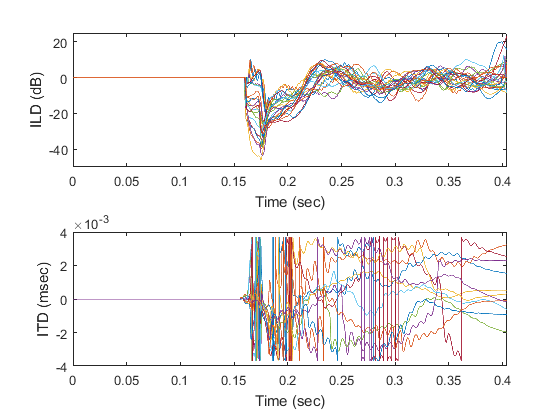
\includegraphics[width=\textwidth]{images/dietz_out_final.png}
  \caption{Τελικές έξοδοι του μοντέλου: (Πάνω) ILD για 23 συχνοτικές μπάντες, (Κάτω) ITD για την δομή envelope - 11 μπάντες.}
  \label{fig:dietz_out_final}
\end{figure}
